\ifx\pdfminorversion\undefined\else\pdfminorversion=4\fi
\documentclass[aspectratio=169,t]{beamer}
%\documentclass[aspectratio=169,t,handout]{beamer}

% English version FAU Logo
\usepackage[english]{babel}
% German version FAU Logo
%\usepackage[ngerman]{babel}

\usepackage[utf8]{inputenc}
\usepackage[T1]{fontenc}
\usepackage{amsmath,amssymb}
\usepackage{graphicx}
\usepackage{listings}
\usepackage{url}
\usepackage{enumitem}
\usepackage{hyperref}
\usepackage{fontawesome}
\usepackage{graphicx}
\usepackage{booktabs}
\usepackage{calc}
\usepackage{ifthen}
\usepackage{xcolor}
\usepackage{tabularx}
\usepackage{tikz}
\usepackage{tikz}
\usepackage{tikz-cd}
\usepackage{verbatim}
\usepackage{pgfplots,pgfplotstable,pgf-pie}
\usepackage{filecontents}
\newcommand{\plots}{0.611201}
\newcommand{\plotm}{2.19882}
\pgfplotsset{height=4cm,width=8cm,compat=1.17}
\pgfmathdeclarefunction{gauss}{2}{%
  \pgfmathparse{1/(#2*sqrt(2*pi))*exp(-((x-#1)^2)/(2*#2^2))}%
}

\tikzset{
    vertex/.style = {
        circle,
        fill            = black,
        outer sep = 2pt,
        inner sep = 1pt,
    }
}
\usetikzlibrary{arrows,decorations.pathmorphing,backgrounds,fit,positioning,shapes.symbols,chains,intersections,snakes,positioning,matrix,mindmap,shapes.multipart,shapes,calc}
\tikzset{level 1/.append style={sibling angle=50,level distance = 165mm}}
\tikzset{level 2/.append style={sibling angle=20,level distance = 45mm}}
\tikzset{every node/.append style={scale=1}}
% read in data file
\pgfplotstableread{data/iris.dat}\iris
% get number of data points
\pgfplotstablegetrowsof{\iris}
\pgfmathsetmacro\NumRows{\pgfplotsretval-1}
\definecolor{airforceblue}{rgb}{0.36, 0.54, 0.66}
\usepgfplotslibrary{groupplots}
\pgfplotsset{compat=1.14}
\newcommand{\tikzmark}[1]{\tikz[remember picture] \node[coordinate] (#1) {#1};}
% Options:
%  - inst:      Institute
%                 med:      MedFak FAU theme
%                 nat:      NatFak FAU theme
%                 phil:     PhilFak FAU theme
%                 rw:       RWFak FAU theme
%                 rw-jura:  RWFak FB Jura FAU theme
%                 rw-wiso:  RWFak FB WISO FAU theme
%                 tf:       TechFak FAU theme
%  - image:     Cover image on title page
%  - plain:     Plain title page
%  - longtitle: Title page layout for long title
\usetheme[%
  image,%
  longtitle,%
  tf
]{fau}

% Enable semi-transparent animation preview
\setbeamercovered{transparent}


\lstset{%
  language=Python,
  tabsize=2,
  basicstyle=\tt,
  keywordstyle=\color{blue},
  commentstyle=\color{green!50!black},
  stringstyle=\color{red},
  numbers=left,
  numbersep=0.5em,
  xleftmargin=1em,
  numberstyle=\tt
}


% Title, authors, and date
\title[KDD]{Chapter IV: OLAP}
\subtitle{Knowledge Discovery in Databases}
\author[L.~Melodia]{Luciano Melodia M.A.}
% English version
\institute[Department]{Evolutionary Data Management, Friedrich-Alexander University Erlangen-Nürnberg}
% German version
%\institute[Lehrstuhl]{Lehrstuhl, Friedrich-Alexander-Universit\"at Erlangen-N\"urnberg}
\date{Summer semester 2021}
% Set additional logo (overwrites FAU seal)
%\logo{\includegraphics[width=.15\textwidth]{themefau/art/xxx/xxx.pdf}}
\begin{document}
  % Title
  \maketitle

  { 
    \setbeamertemplate{footline}{}
    \begin{frame}{Chapter IV: Data warehousing and online analytical processing}
        \begin{itemize}
            \item \textbf{Data warehouse: basic concepts.}
            \item Data-warehouse modeling: data cube and OLAP.
            \item Data-warehouse design and usage.
            \item Data-warehouse Implementation.
            \item Data generalization by attribute-oriented induction.
            \item Summary.
        \end{itemize}
    \end{frame}
  }

  { 
    \setbeamertemplate{footline}{}
    \begin{frame}{What is a data warehouse?}
        \begin{itemize}
            \item \textbf{Defined in many different ways, but not rigorously:}
            \begin{itemize}
              \item A \textbf{\color{airforceblue}decision-support} database that is \textbf{\color{airforceblue}maintained separately} from the organization's operational database.
              \item Supports information processing by providing a solid platform of \textbf{\color{airforceblue}consolidated, historical data} for analysis.
            \end{itemize}
            \item \textbf{Famous:} \\
            \emph{A data warehouse is a {\color{airforceblue}subject-oriented, integrated, time-variant, and nonvolatile} collection of data in support of management's decision-making process.} \\
            -- W. H. Inmon.
            \item \textbf{\color{airforceblue}Data warehousing:} The process of constructing and using data warehouses.
        \end{itemize}
    \end{frame}
  }

  { 
    \setbeamertemplate{footline}{}
    \begin{frame}{Data warehouse -- subject-oriented}
        \begin{itemize}
            \item \textbf{Organized around major subjects.}
            \begin{itemize}
              \item Such as customer, product, sales.
            \end{itemize}
            \item \textbf{Focusing on the modeling and analysis of data for {\color{airforceblue}decision makers}.}
            \begin{itemize}
              \item Not on daily operations or transaction processing.
            \end{itemize}
            \item \textbf{Provide a simple and concise view around particular subject issues.}
            \begin{itemize}
              \item By excluding data that are not useful in the decision-support process.
            \end{itemize}
        \end{itemize}
    \end{frame}
  }

  { 
    \setbeamertemplate{footline}{}
    \begin{frame}{Data warehouse -- integrated}
        \begin{itemize}
            \item \textbf{Constructed by {\color{airforceblue}integrating multiple heterogeneous data sources}.}
            \begin{itemize}
              \item Relational databases, flat files, online transaction records, \ldots
            \end{itemize}
            \item \textbf{Data-cleaning and data-integration techniques are applied.}
            \begin{itemize}
              \item Ensure consistency in naming conventions, encoding structures, attribute measures, etc. among different data sources.
              \item E.g., hotel price: currency, tax, breakfast covered, etc.
              \item When data is moved to the warehouse, it is converted.
              \item ETL -- Extraction, Transformation, Loading, see below.
            \end{itemize}
        \end{itemize}
    \end{frame}
  }

  { 
    \setbeamertemplate{footline}{}
    \begin{frame}{Data warehouse -- time variant}
        \begin{itemize}
            \item \textbf{The {\color{airforceblue}time horizon} for a data warehouse is {\color{airforceblue}significantly longer} than that of operational systems.}
            \begin{itemize}
              \item Operational database: current-value data.
            \end{itemize}
            \item Data warehouse: provide information from a historical perspective, e.g. past $5-10$ years.
            \item \textbf{Every key structure in the data warehouse contains \\
            an element of time, explicitly or implicitly.}
            \item The key of operational data may or may not contain a "time element."
        \end{itemize}
    \end{frame}
  }

  { 
    \setbeamertemplate{footline}{}
    \begin{frame}{Data warehouse -- nonvolatile}
        \begin{itemize}
            \item \textbf{A {\color{airforceblue}physically separate} store of data.}
            \begin{itemize}
              \item Transformed from the operational environment.
              \item By {\color{airforceblue}copying}.
            \end{itemize}
            \item \textbf{No operational update of data:}
            \begin{itemize}
              \item Hence, does not require transaction processing, \\
              i.e. no logging, recovery, concurrency control, etc.
              \item Requires only three operations:
              \begin{itemize}
                \item Initial loading of data.
                \item Refresh (update, often periodically, e.g. over night).
                \item Access of data.
              \end{itemize}
            \end{itemize}
        \end{itemize}
    \end{frame}
  }

  { 
    \setbeamertemplate{footline}{}
    \begin{frame}{OLTP vs. OLAP}
      \begin{tabularx}{\textwidth}{|l|X|X|}
      & \textbf{OLTP} & \textbf{OLAP} \\\hline
      \textbf{users} & clerk, IT professional & knowledge worker \\
      \textbf{function} & day-to-day operations & decision support \\
      \textbf{DB design} & application-oriented & decision support \\
      \textbf{data} & current, up-to-date; detailed, flat relational; isolated & historical; summarized, multidimensional, integrated, consolidated \\
      \textbf{usage} & repetitive & ad-hoc \\
      \textbf{access} & read/write; index/hash on primary key & lots of scans \\
      \textbf{unit of work} & short, simple transaction & complex query \\
      \textbf{$\#$-records accessed} & $~ 10$ & $~ 10^6$ \\
      \textbf{$\#$-users} & $~ 1000$ & $~ 100$ \\
      \textbf{DB size} & $~ 100$ MB to GB & $~ 100$ GB to TB \\
      \textbf{quantification} & transaction throughput & query throughput, response \\
      \end{tabularx}
    \end{frame}
  }

  { 
    \setbeamertemplate{footline}{}
    \begin{frame}{Why a separate data warehouse?}
    \begin{itemize}
      \item \textbf{High performance for both systems:}
      \begin{itemize}
        \item \textbf{\color{airforceblue}DBMS}: tuned for OLTP; Access methods, indexing concurreny control, recovery.
        \item \textbf{\color{airforceblue}Warehouse}: tuned for OLAP; Complex OLAP queries, multidimensional view, consolidation.
      \end{itemize}
      \item \textbf{Different functions and different data:}
      \begin{itemize}
        \item Missing data:
        \begin{itemize}
          \item Decision support (DS) requires \textbf{\color{airforceblue}historical data} \\ which operational DBs do not typically maintain.
        \end{itemize}
        \item Data consolidation:
        \begin{itemize}
          \item DS requires \textbf{\color{airforceblue}consolidation} (aggregation, summarization) \\
          of data from heterogeneous sources.
        \end{itemize}
        \item Data quality:
        \begin{itemize}
          \item Different sources typically use inconsistent data representations, \\ codes and formats which have to be reconciled.
        \end{itemize}
      \end{itemize}
      \item \textbf{Note: There are more and more systems which perform OLAP\\ analysis directly on relational databases.}
    \end{itemize}
    \end{frame}
  }

  { 
    \setbeamertemplate{footline}{}
    \begin{frame}{}

    \end{frame}
  }

  { 
    \setbeamertemplate{footline}{}
    \begin{frame}{Three data-warehouse models}
    \begin{itemize}
      \item \textbf{\color{airforceblue}Enterprise Warehouse:}
      \begin{itemize}
        \item Collects all of the information about subjects spanning the entire organization.
      \end{itemize}
      \item \textbf{\color{airforceblue}Data mart:}
      \begin{itemize}
        \item A \textbf{\color{airforceblue}subset} of corporate-wide data that is of value to a \textbf{\color{airforceblue}specific group of users.}
        \item Its scope is confined to specific, selected groups, such as marketing data mart.
        \item Independent vs. dependent (directly from warehouse) data mart.
      \end{itemize}
      \item \textbf{\color{airforceblue}Virtual warehouse:}
       \begin{itemize}
        \item A set of \textbf{\color{airforceblue}views} over operational databases.
        \item Only some of the possible summary views may be materialized.
      \end{itemize}
   \end{itemize}
    \end{frame}
  }
  
  { 
    \setbeamertemplate{footline}{}
    \begin{frame}{Extraction, transformation, and loading (ETL)}
    \begin{itemize}
      \item \textbf{\color{airforceblue}Extraction:}
      \begin{itemize}
        \item Get data from multiple, heterogeneous, and external sources.
      \end{itemize}
      \item \textbf{\color{airforceblue}Cleaning:}
      \begin{itemize}
        \item Detect errors in the data and rectify them if possible.
      \end{itemize}
      \item \textbf{\color{airforceblue}Transformation:}
      \begin{itemize}
        \item Convert data from legacy or host format to warehouse format.
      \end{itemize}
      \item \textbf{\color{airforceblue}Loading:}
      \begin{itemize}
        \item Sort, summarize, consolidate, compute views, check integrity, and build indexes and partitions.
      \end{itemize}
      \item \textbf{\color{airforceblue}Refresh:}
      \begin{itemize}
        \item Propagate only the updates from the data sources to the warehouse.
      \end{itemize}
    \end{itemize}
    \end{frame}
  }

  { 
    \setbeamertemplate{footline}{}
    \begin{frame}{Metadata repository}
    \begin{itemize}
      \item \textbf{Metadata: the data defining data-warehouse objects.}
      \item \textbf{Description of the {\color{airforceblue}structure} of the data warehouse:}
      \begin{itemize}
        \item Schema, view, dimensions, hierarchies, derived-data definition, data-mart locations and contents.
      \end{itemize}
      \item \textbf{{\color{airforceblue}Operational} metadata:}
      \begin{itemize}
        \item \textbf{\color{airforceblue}Data lineage} (history of migrated data and transformation path).
        \item Currency of data (active, archived, or purged).
        \item Monitoring information (warehouse-usage statistics, error reports, audit trails).
      \end{itemize}
      \item \textbf{{\color{airforceblue}Algorithms} used for summarization.}
      \item \textbf{{\color{airforceblue}Mapping} from operational environment to data warehouse.}
      \item \textbf{Data related to system performance:}
      \begin{itemize}
        \item Warehouse schema, view and derived-data definitions.
      \end{itemize}
      \item \textbf{Business data:}
      \begin{itemize}
        \item Business terms and definitions, ownership of data, charging policies.
      \end{itemize}
    \end{itemize}
    \end{frame}
  }

  { 
    \setbeamertemplate{footline}{}
    \begin{frame}{Chapter IV: Data warehousing and online analytical processing}
        \begin{itemize}
            \item Data warehouse: basic concepts.
            \item \textbf{Data-warehouse modeling: data cube and OLAP.}
            \item Data-warehouse design and usage.
            \item Data-warehouse Implementation.
            \item Data generalization by attribute-oriented induction.
            \item Summary.
        \end{itemize}
    \end{frame}
  }

  { 
    \setbeamertemplate{footline}{}
    \begin{frame}{From tables and spreadsheets to data cubes}
        \begin{itemize}
            \item Data warehouse: basic concepts.
            \begin{itemize}
              \item Based on a \textbf{\color{airforceblue}multidimensional data model} which views data in the form of a \textbf{data cube}.
            \end{itemize}
            \item \textbf{Data cube.}
            \begin{itemize}
              \item Allows data (here: sales) to be modeled and viewed in multiple dimensions.
              \begin{itemize}
                \item \textbf{Dimension tables:} such as: \texttt{item (item\_name, brand, type)},\\
                or: \texttt{time (day, week, month, quarter, year)}.
                \item \textbf{Fact table:} Contains \textbf{measures} (such as \texttt{dollars\_sold}) and references (\texttt{foreign keys}) to each of the related dimension tables.
              \end{itemize}
            \end{itemize}
            \item \textbf{$n$-dimensional base cube.}
            \begin{itemize}
              \item Called a base cuboid in data-warehousing literature.
            \end{itemize}
            \item \textbf{Top most $0$-dimensional cuboid.}
            \begin{itemize}
              \item Holds the highest-level of summarization.
              \item Called the apex cuboid.
            \end{itemize}
            \item \textbf{Lattice of cuboids.} (Forms a data cube)
        \end{itemize}
    \end{frame}
  }

  { 
    \setbeamertemplate{footline}{}
    \begin{frame}{Cube: a lattice of cuboids}
    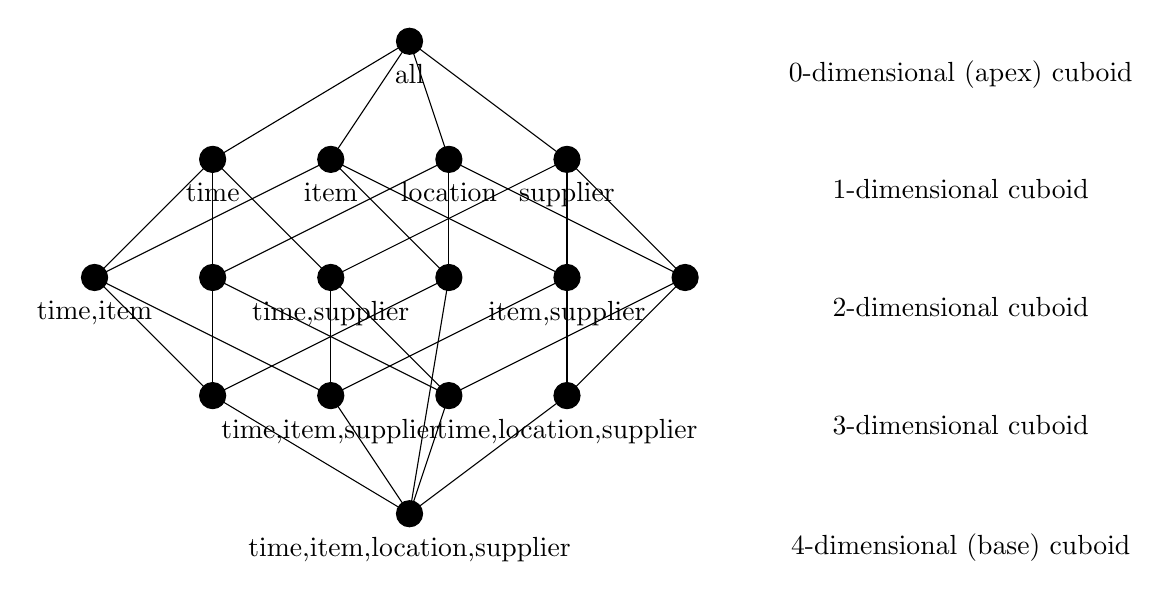
\begin{tikzpicture}
      \node[draw, circle, fill=black, label=below:{all}] at (2,6) {};
      \draw (2,6) -- (-0.5,4.5);
      \draw (2,6) -- (1,4.5);
      \draw (2,6) -- (2.5,4.5);
      \draw (2,6) -- (4,4.5);

      \node[draw, circle, fill=black, label=below:{time}] at (-0.5,4.5) {};
      \node[draw, circle, fill=black, label=below:{item}] at (1,4.5) {};
      \node[draw, circle, fill=black, label=below:{location}] at (2.5,4.5) {};
      \node[draw, circle, fill=black, label=below:{supplier}] at (4,4.5) {};
      \draw (-0.5,4.5) -- (-2,3);
      \draw (-0.5,4.5) -- (-0.5,3);
      \draw (-0.5,4.5) -- (1,3);
      \draw (1,4.5) -- (-2,3);
      \draw (1,4.5) -- (2.5,3);
      \draw (1,4.5) -- (4,3);
      \draw (2.5,4.5) -- (-0.5,3);
      \draw (2.5,4.5) -- (2.5,3);
      \draw (2.5,4.5) -- (5.5,3);
      \draw (4,4.5) -- (1,3);
      \draw (4,4.5) -- (4,3);
      \draw (4,4.5) -- (5.5,3);


      \node[draw, circle, fill=black, label=below:{time,item}] at (-2,3) {};
      \node[draw, circle, fill=black] at (-0.5,3) {};
      \node[draw, circle, fill=black, label=below:{time,supplier}] at (1,3) {};
      \node[draw, circle, fill=black] at (2.5,3) {};
      \node[draw, circle, fill=black, label=below:{item,supplier}] at (4,3) {};
      \node[draw, circle, fill=black] at (5.5,3) {};
      \draw (-2,3) -- (-0.5,1.5);
      \draw (-2,3) -- (1,1.5);
      \draw (-0.5,3) -- (-0.5,1.5);
      \draw (-0.5,3) -- (2.5,1.5);
      \draw (1,3) -- (1,1.5);
      \draw (1,3) -- (2.5,1.5);
      \draw (2.5,3) -- (-0.5,1.5);
      \draw (2.5,3) -- (2,0);
      \draw (4,3) -- (1,1.5);
      \draw (4,3) -- (4,1.5);
      \draw (5.5,3) -- (2.5,1.5);
      \draw (5.5,3) -- (4,1.5);

      \node[draw, circle, fill=black] at (-0.5,1.5) {};
      \node[draw, circle, fill=black, label=below:{time,item,supplier}] at (1,1.5) {};
      \node[draw, circle, fill=black] at (2.5,1.5) {};
      \node[draw, circle, fill=black, label=below:{time,location,supplier}] at (4,1.5) {};
      \draw (-0.5,1.5) -- (2,0);
      \draw (1,1.5) -- (2,0);
      \draw (2.5,1.5) -- (2,0);
      \draw (4,1.5) -- (2,0);

      \node[draw, circle, fill=black, label=below:{time,item,location,supplier}] at (2,0)  {};

      \node[label=below:{$0$-dimensional (apex) cuboid}] at (9,6)  {};
      \node[label=below:{$1$-dimensional cuboid}] at (9,4.5)  {};
      \node[label=below:{$2$-dimensional cuboid}] at (9,3)  {};
      \node[label=below:{$3$-dimensional cuboid}] at (9,1.5)  {};
      \node[label=below:{$4$-dimensional (base) cuboid}] at (9,0)  {};
    \end{tikzpicture}
    \end{frame}
  }

  { 
    \setbeamertemplate{footline}{}
    \begin{frame}{Conceptual modeling of data warehouses}
        \begin{itemize}
            \item \textbf{Star schema:}.
            \begin{itemize}
                \item A fact table in the middle connected to a set of dimension tables.
            \end{itemize}
            \item \textbf{Snowflake schema:}.
            \begin{itemize}
                \item A refinement of the star schema where some dimensional hierarchy \\
                 is \textbf{normalized} into a set of smaller dimension tables,\\
                forming a shape similar to a snowflake.
            \end{itemize}
            \item \textbf{Fact constellations:}.
            \begin{itemize}
                \item Multiple fact tables sharing dimension tables, \\
                viewed as a collection of stars, therefore called \\
                \textbf{galaxy schema} or fact constellation.
            \end{itemize}
        \end{itemize}
    \end{frame}
  }

  { 
    \setbeamertemplate{footline}{}
    \begin{frame}{Example of star schema}
    \tikzset{basic/.style={
            draw,
            rectangle split,
            rectangle split parts=2,
            rectangle split part fill={blue!20,white},
            minimum width=2.5cm,
            text width=2cm,
            align=left,
            font=\itshape
        },
        Diamond/.style={ diamond, 
                         draw, 
                            shape aspect=2, 
                            inner sep = 2pt,
                            text centered,
                            fill=blue!10!white,
                            font=\itshape
                          }}
    \begin{tikzpicture}
    \node[basic, rectangle split part fill={green!20,white}] at (2,2) (time) {time
    \nodepart{second}
    \underline{time\_key}\\
    day\\
    day\_of\_week\\
    month\\
    quarter\\
    year};

    \node[basic] at (2,-2) (branch) {branch
    \nodepart{second}
    \underline{branch\_key}\\
    branch\_name\\
    branch\_type};

    \node[basic, rectangle split part fill={orange!20,white}] at (12,2) (item) {item
    \nodepart{second}
    \underline{item\_key}\\
    item\_name\\
    brand\\
    type\\
    supplier\_type};

    \node[basic, rectangle split part fill={yellow!20,white}] at (12,-1.5) (location) {location
    \nodepart{second}
    \underline{location\_key}\\
    street\\
    city\\
    province\\
    country};

    \node[] at (7,3) {Sales fact table:};
    \node[fill=green!20, minimum width = 3cm, minimum height=0.5cm, align=right] at (7,2.5) (a) {time\_key};
    \node[fill=orange!20, minimum width = 3cm, minimum height=0.5cm, align=right] at (7,2) (b) {item\_key};
    \node[fill=blue!20, minimum width = 3cm, minimum height=0.5cm, align=right] at (7,1.5) (c) {branch\_key};
    \node[fill=yellow!20, minimum width = 3cm, minimum height=0.5cm, align=right] at (7,1) (d) {location\_key};
    \node[fill=red!20, minimum width = 3cm, minimum height=0.5cm, align=right] at (7,0.5) (units) {units\_sold};
    \node[fill=red!20, minimum width = 3cm, minimum height=0.5cm, align=right] at (7,0) (dollars) {dollars\_sold};
    \node[fill=red!20, minimum width = 3cm, minimum height=0.5cm, align=right] at (7,-0.5) (sales) {avg\_sales};
    \draw[->, dashed] (a) -- (time) ;
    \draw[->, dashed] (b) -- (item) ;
    \draw[->, dashed] (c) -- (branch) ;
    \draw[->, dashed] (d) -- (location) ;

    \node[fill=red!20, minimum width = 3cm, minimum height=0.5cm, align=right] at (5,-1.5) (e) {Measures};
    \draw[-] (e) -- (units) ;
    \draw[-] (e) -- (dollars) ;
    \draw[-] (e) -- (sales) ;
    \end{tikzpicture}
    \end{frame}
  }

  { 
    \setbeamertemplate{footline}{}
    \begin{frame}{Example of snowflake schema}
    \tikzset{basic/.style={
            draw,
            rectangle split,
            rectangle split parts=2,
            rectangle split part fill={blue!20,white},
            minimum width=2.5cm,
            text width=2cm,
            align=left,
            font=\itshape
        },
        Diamond/.style={ diamond, 
                         draw, 
                            shape aspect=2, 
                            inner sep = 2pt,
                            text centered,
                            fill=blue!10!white,
                            font=\itshape
                          }}
    \begin{tikzpicture}
    \node[basic, rectangle split part fill={green!20,white}] at (2,2) (time) {time
    \nodepart{second}
    \underline{time\_key}\\
    day\\
    day\_of\_week\\
    month\\
    quarter\\
    year};

    \node[basic] at (2,-2) (branch) {branch
    \nodepart{second}
    \underline{branch\_key}\\
    branch\_name\\
    branch\_type};

    \node[basic, rectangle split part fill={orange!20,white}] at (10,2) (item) {item
    \nodepart{second}
    \underline{item\_key}\\
    item\_name\\
    brand\\
    type\\
    supplier\_key};

    \node[basic, rectangle split part fill={orange!20,white}] at (13,2) (supplier) {supplier
    \nodepart{second}
    \underline{supplier\_key}\\
    supplier\_type};

    \node[basic, rectangle split part fill={yellow!20,white}] at (10,-1.5) (location) {location
    \nodepart{second}
    \underline{location\_key}\\
    street\\
    city\_key};

    \node[basic, rectangle split part fill={yellow!20,white}] at (13,-1.5) (city) {city
    \nodepart{second}
    \underline{city\_key}\\
    city\\
    province\\
    country};

    \node[] at (6,3) {Sales fact table:};
    \node[fill=green!20, minimum width = 3cm, minimum height=0.5cm, align=right] at (6,2.5) (a) {time\_key};
    \node[fill=orange!20, minimum width = 3cm, minimum height=0.5cm, align=right] at (6,2) (b) {item\_key};
    \node[fill=blue!20, minimum width = 3cm, minimum height=0.5cm, align=right] at (6,1.5) (c) {branch\_key};
    \node[fill=yellow!20, minimum width = 3cm, minimum height=0.5cm, align=right] at (6,1) (d) {location\_key};
    \node[fill=red!20, minimum width = 3cm, minimum height=0.5cm, align=right] at (6,0.5) (units) {units\_sold};
    \node[fill=red!20, minimum width = 3cm, minimum height=0.5cm, align=right] at (6,0) (dollars) {dollars\_sold};
    \node[fill=red!20, minimum width = 3cm, minimum height=0.5cm, align=right] at (6,-0.5) (sales) {avg\_sales};
    \draw[->, dashed] (a) -- (time) ;
    \draw[->, dashed] (b) -- (item) ;
    \draw[->, dashed] (c) -- (branch) ;
    \draw[->, dashed] (d) -- (location) ;
    \draw[->, dashed] (10,-2) -- (city) ;
    \draw[->, dashed] (11,1) -- (supplier) ;

    \node[fill=red!20, minimum width = 3cm, minimum height=0.5cm, align=right] at (5,-1.5) (e) {Measures};
    \draw[-] (e) -- (units) ;
    \draw[-] (e) -- (dollars) ;
    \draw[-] (e) -- (sales) ;
    \end{tikzpicture}
    \end{frame}
  }

  { 
    \setbeamertemplate{footline}{}
    \begin{frame}{Example of fact constellation}
    \tikzset{basic/.style={
            draw,
            rectangle split,
            rectangle split parts=2,
            rectangle split part fill={blue!20,white},
            minimum width=2.5cm,
            text width=2cm,
            align=left,
            font=\itshape
        },
        Diamond/.style={ diamond, 
                         draw, 
                            shape aspect=2, 
                            inner sep = 2pt,
                            text centered,
                            fill=blue!10!white,
                            font=\itshape
                          }}
    \begin{tikzpicture}
    \node[basic, rectangle split part fill={green!20,white}] at (2,2) (time) {time
    \nodepart{second}
    \underline{time\_key}\\
    day\\
    day\_of\_week\\
    month\\
    quarter\\
    year};

    \node[basic] at (2,-2) (branch) {branch
    \nodepart{second}
    \underline{branch\_key}\\
    branch\_name\\
    branch\_type};

    \node[basic, rectangle split part fill={orange!20,white}] at (10,2) (item) {item
    \nodepart{second}
    \underline{item\_key}\\
    item\_name\\
    brand\\
    type\\
    supplier\_type};

    \node[basic, rectangle split part fill={yellow!20,white}] at (10,-1.5) (location) {location
    \nodepart{second}
    \underline{location\_key}\\
    street\\
    city\\
    province\\
    country};

    \node[basic, rectangle split part fill={blue!20,white}] at (13.5,-2) (shipper) {shipper
    \nodepart{second}
    \underline{shipper\_key}\\
    shipper\_name\\
    location\_key\\
    shipper\_type};

    \node[] at (6,3) {Sales fact table:};
    \node[fill=green!20, minimum width = 3cm, minimum height=0.5cm, align=right] at (6,2.5) (a) {time\_key};
    \node[fill=orange!20, minimum width = 3cm, minimum height=0.5cm, align=right] at (6,2) (b) {item\_key};
    \node[fill=blue!20, minimum width = 3cm, minimum height=0.5cm, align=right] at (6,1.5) (c) {branch\_key};
    \node[fill=yellow!20, minimum width = 3cm, minimum height=0.5cm, align=right] at (6,1) (d) {location\_key};
    \node[fill=red!20, minimum width = 3cm, minimum height=0.5cm, align=right] at (6,0.5) (units) {units\_sold};
    \node[fill=red!20, minimum width = 3cm, minimum height=0.5cm, align=right] at (6,0) (dollars) {dollars\_sold};
    \node[fill=red!20, minimum width = 3cm, minimum height=0.5cm, align=right] at (6,-0.5) (sales) {avg\_sales};
    \draw[->, dashed] (a) -- (time) ;
    \draw[->, dashed] (b) -- (item) ;
    \draw[->, dashed] (c) -- (branch) ;
    \draw[->, dashed] (d) -- (location) ;


    \node[] at (13.5,3) {Shipping fact table:};
    \node[fill=green!20, minimum width = 3cm, minimum height=0.5cm, align=right] at (13.5,2.5) (q) {time\_key};
    \node[fill=orange!20, minimum width = 3cm, minimum height=0.5cm, align=right] at (13.5,2) (w) {item\_key};
    \node[fill=blue!20, minimum width = 3cm, minimum height=0.5cm, align=right] at (13.5,1.5) (e) {shipper\_key};
    \node[fill=yellow!20, minimum width = 3cm, minimum height=0.5cm, align=right] at (13.5,1) (r) {from\_location};
    \node[fill=yellow!20, minimum width = 3cm, minimum height=0.5cm, align=right] at (13.5,0.5) (t) {to\_location};
    \node[fill=red!20, minimum width = 3cm, minimum height=0.5cm, align=right] at (13.5,0) (z) {dollars\_cost};
    \node[fill=red!20, minimum width = 3cm, minimum height=0.5cm, align=right] at (13.5,-0.5) (u) {units\_shipped};
    \draw[->, dashed] (q) -- (time) ;
    \draw[->, dashed] (w) -- (item) ;
    \draw[->, dashed] (e) to [out=30,in=30] (shipper) ;
    \draw[->, dashed] (r) -- (location) ;
    \draw[->, dashed] (t) -- (location) ;
    \draw[->, dashed] (shipper) -- (location) ;

    \node[fill=red!20, minimum width = 3cm, minimum height=0.5cm, align=right] at (5,-1.5) (e) {Measures};
    \draw[-] (e) -- (units) ;
    \draw[-] (e) -- (dollars) ;
    \draw[-] (e) -- (sales) ;
    \end{tikzpicture}
    \end{frame}
  }

  { 
    \setbeamertemplate{footline}{}
    \begin{frame}{A concept hierarchy: dimension (location)}
    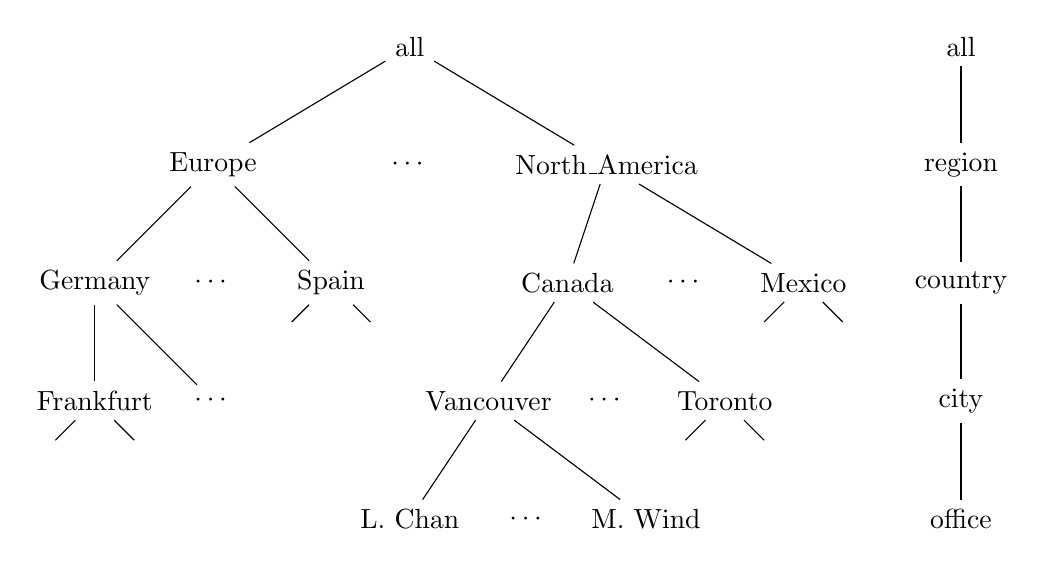
\begin{tikzpicture}
      \node at (2,6) (all) {all};

      \node at (-0.5,4.5) (europe) {Europe};
      \node at (2,4.5) (dot1) {$\cdots$};
      \node at (4.5,4.5) (america) {North\_America};

      \node at (-2,3) (germany) {Germany};
      \node at (-0.5,3) (dots2) {$\cdots$};
      \node at (1,3) (spain) {Spain};
      \node at (4,3) (canada) {Canada};
      \node at (5.5,3) (dots3) {$\cdots$};
      \node at (7,3) (mexico) {Mexico};

      \node at (-2,1.5) (frankfurt) {Frankfurt};
      \node at (-0.5,1.5) (dots4) {$\cdots$};
      \node at (3,1.5) (vancouver) {Vancouver};
      \node at (4.5,1.5) (dots5) {$\cdots$};
      \node at (6,1.5) (toronto) {Toronto};
      \node at (2,0) (lchan) {L. Chan};
      \node at (3.5,0) (dots6) {$\cdots$};
      \node at (5,0) (mwind) {M. Wind};

      \draw (all) -- (europe);
      \draw (all) -- (america);
      \draw (europe) -- (germany);
      \draw (europe) -- (spain);
      \draw (america) -- (canada);
      \draw (america) -- (mexico);
      \draw (germany) -- (frankfurt);
      \draw (germany) -- (dots4);
      \draw (spain) -- (0.5,2.5);
      \draw (spain) -- (1.5,2.5);
      \draw (mexico) -- (6.5,2.5);
      \draw (mexico) -- (7.5,2.5);
      \draw (frankfurt) -- (-2.5,1);
      \draw (frankfurt) -- (-1.5,1);
      \draw (toronto) -- (5.5,1);
      \draw (toronto) -- (6.5,1);
      \draw (canada) -- (vancouver);
      \draw (canada) -- (toronto);
      \draw (vancouver) -- (lchan);
      \draw (vancouver) -- (mwind);

      \node at (9,6) (all2) {all};
      \node at (9,4.5) (region2)  {region};
      \node at (9,3) (country2) {country};
      \node at (9,1.5) (city2) {city};
      \node at (9,0) (office2) {office};
      \draw (all2) -- (region2);
      \draw (region2) -- (country2);
      \draw (country2) -- (city2);
      \draw (city2) -- (office2);
    \end{tikzpicture}
    \end{frame}
  }

  { 
    \setbeamertemplate{footline}{}
    \begin{frame}{Data-cube measures: three categories}
        \begin{itemize}
            \item \textbf{Distributive:}
            \begin{itemize}
              \item If the result derived by applying the function to the $n$ aggregate values obtained for $n$ partitions of the dataset is the same as that derived by applying the function on all the data without partitioning.\\
              E.g. \texttt{COUNT, SUM, MIN, MAX}.
            \end{itemize}
            \item \textbf{Functional:}
            \begin{itemize}
              \item If it can be computed by an algebraic function with $M$ arguments, each of which is obtained by applying a distributive aggregate function.\\
              E.g. \texttt{AVG, MIN$_N$, STD}.
            \end{itemize}
            \item \textbf{Holistic:}
            \begin{itemize}
              \item If there is no constant bound on the storage size needed to describe a subaggregate.\\
              E.g. \texttt{MEDIAN, MODE, RANK}.
            \end{itemize}
        \end{itemize}
    \end{frame}
  }

  { 
    \setbeamertemplate{footline}{}
    \begin{frame}{Aggregation type}
        \begin{itemize}
            \item \textbf{Non-trivial property.}
            \begin{itemize}
              \item Next to name and value range.
            \end{itemize}
            \item \textbf{Defines the set of aggregation operations that can be executed on a measure (a fact).}
            \item \textbf{\color{airforceblue}FLOW:}
            \begin{itemize}
              \item Any aggregation.
              \item E.g. sales turnover.
            \end{itemize}
            \item \textbf{\color{airforceblue}STOCK:}
            \begin{itemize}
              \item No temporal aggregation.
              \item E.g. stock, inventory.
            \end{itemize}
            \item \textbf{\color{airforceblue}VPU (Value per Unit:}
            \begin{itemize}
              \item No summarization.
              \item E.g. price, tax, in general factors.
            \end{itemize}
            \item \textbf{(Always applicable: \texttt{MIN}, \texttt{MAX} and \texttt{AVG}).}
        \end{itemize}
    \end{frame}
  }


  { 
    \setbeamertemplate{footline}{}
    \begin{frame}{Chapter IV: Data warehousing and online analytical processing}
        \begin{itemize}
            \item Data warehouse: basic concepts.
            \item Data-warehouse modeling: data cube and OLAP.
            \item Data-warehouse design and usage.
            \item Data-warehouse Implementation.
            \item \textbf{Data generalization by attribute-oriented induction.}
            \item Summary.
        \end{itemize}
    \end{frame}
  }

  { 
    \setbeamertemplate{footline}{}
    \begin{frame}{Data generalization}
    \begin{itemize}
      \item \textbf{Summarize data:}
      \begin{itemize}
        \item \textbf{By replacing relatively low-level values} \\
        e.g. numerical values for the attribute \texttt{age} \\
        \textbf{with higher-level concepts}\\
        e.g. \texttt{young}, \texttt{middle-aged} and \texttt{senior}.
        \item \textbf{By reducing the number of dimensions}\\
              e.g. removing \texttt{birth\_date} and \texttt{telephone\_number} \\ when summarizing the behavior of a group of students.
        \item Describe concepts in concise and succinct terms at generalized (rather than low) levels of abstractions:
        \begin{itemize}
          \item Facilitates users in examining the general behavior of the data.
          \item Makes dimensions of a data cube easier to grasp.
        \end{itemize}
      \end{itemize}
    \end{itemize}
    \end{frame}
  }

  { 
    \setbeamertemplate{footline}{}
    \begin{frame}{Attribute-oriented induction}
    \begin{itemize}
      \item \textbf{Proposed in 1989} (KDD'89 workshop).
      \item \textbf{Not confined to categorical data nor to particular measures.}
      \item \textbf{How is it done?}
      \begin{itemize}
        \item Collect the \textbf{\color{airforceblue}task-relevant data} (initial relation) using a relational database query.
        \item Perform \textbf{\color{airforceblue}generalization} by attribute removal or attribute generalization.
        \item Apply \textbf{\color{airforceblue}aggregation} by merging identical, generalized tuples and \\ accumulating their respective counts.
        \item Interaction with users for knowledge presentation.
      \end{itemize}
    \end{itemize}
    \end{frame}
  }

  { 
    \setbeamertemplate{footline}{}
    \begin{frame}{Attribute-oriented induction: an example}
    \begin{itemize}
      \item \textbf{Example:} Describe general characteristics of graduate students in a University database.
      \item \textbf{Step 1:} Fetch relevant set of data using an SQL statement, e.g.\\[0.1cm]
      \texttt{SELECT name, gender, major, birth\_place, birth\_date, residence, phone\#, gpa)}\\
      \texttt{FROM student}\\
      \texttt{WHERE student\_status IN {"Msc", "MBA", "PhD"};}\\[0.1cm]
      \item \textbf{Step 2:} Perform attribute-oriented induction.
      \item \textbf{Step 3:} Present results in generalized-relation, cross-tab, or rule forms.
    \end{itemize}
    \end{frame}
  }

  { 
    \setbeamertemplate{footline}{}
    \begin{frame}{Class characterization: an initial relation (I)}
    \begin{table}
    \small
    \begin{tabularx}{\textwidth}{|X|X|X|X|X|X|X|X|}
    \hline
    Name & Gender & Major & Birth place & Birth date & Residence & Phone number & GPA \\
    Jim & M & CS & Vancouver, BC, Canada & 08-21-76 & 3511 Main St., Richmond & 687-4598 & 3.67 \\\hline
    Scott Lachance & M & CS & Montreal, Que, Canada & 28-07-75 & 345 1st Ave., Richmond & 253-9106 & 3.70 \\\hline
    Laura Lee & F & Physics & Seattle, WA, USA & 25-08-70 & 125 Austin Ave., Burnaby & 420-5232 & 3.83 \\\hline
    {\color{red}Removed} & {\color{red}Retained} & {\color{red}Sci, Eng, Bus} & {\color{red}Country} & {\color{red}Age range} & {\color{red}City} & {\color{red}Removed} & {\color{red}Excl, Vg,\ldots} \\\hline
    \end{tabularx}
    \end{table}
    \end{frame}
  }

  { 
    \setbeamertemplate{footline}{}
    \begin{frame}{Class characterization: prime generalized relation (II)}
    \begin{table}
    \begin{tabularx}{\textwidth}{|X|X|X|X|X|X|X|}
    \hline
    Gender & Major & Birth region & Age range & Residence & GPA & Count \\\hline
    M & Science & Canada & 20-35 & Richmond & Very good & 16 \\\hline
    F & Science & Foreign & 25-30 & Burnaby & Excellent & 22 \\\hline
    \ldots & \ldots & \ldots & \ldots & \ldots & \ldots & \ldots \\
    \hline
    \end{tabularx}
    \end{table}
    \end{frame}
  }

  { 
    \setbeamertemplate{footline}{}
    \begin{frame}{Class characterization: an example (III)}
    \centering
    Cross-table of birth region and gender:\\[0.5cm]
    \begin{tabular}{|l|c|c|c|}
    \hline
    & Canada & Foreign & Total \\\hline
    M & 16 & 14 & 30 \\\hline
    F & 10 & 22 & 32 \\\hline
    Total & 26 & 36 & 62 \\\hline
    \end{tabular}
    \end{frame}
  }

  { 
    \setbeamertemplate{footline}{}
    \begin{frame}{Basic principles of attribute-oriented induction}
    \begin{itemize}
      \item \textbf{Data focusing:}
      \begin{itemize}
        \item Task-relevant data, including dimensions
        \item The result is the \textbf{\color{airforceblue}initial relation}.
      \end{itemize}
      \item \textbf{\color{airforceblue}Attribute removal:}
      \begin{itemize}
        \item Remove attribute A, if there is a large set of distinct values for A,\\
        but (1) there is no generalization operator on A,\\
        or (2) A's higher-level concepts are expressed in terms of other attributes.
      \end{itemize}
      \item \textbf{\color{airforceblue}Attribute generalization:}
      \begin{itemize}
        \item If there is a large set of distinct values for A,\\
              and there exists a \textbf{\color{airforceblue}set of generalization operators} on A,\\
              then select an operator and generalize A.
      \end{itemize}
      \item \textbf{Attribute-threshold control:}
      \begin{itemize}
        \item Typical 2-8, specified/default.
      \end{itemize}
      \item \textbf{Generalized-relation-threshold control:}
      \begin{itemize}
        \item Control the final relation/rule size.
      \end{itemize}
    \end{itemize}
    \end{frame}
  }

  { 
    \setbeamertemplate{footline}{}
    \begin{frame}{Attribute-oriented induction: basic algorithm }
    \begin{itemize}
      \item \textbf{InitialRel:}
      \begin{itemize}
        \item Query processing of task-relevant data, deriving the initial relation.
      \end{itemize}
      \item \textbf{PreGen:}
      \begin{itemize}
        \item Based on the analysis of the number of distinct values in each attribute, determine generalization plan for each attribute: removal? Or how high to generalize?
      \end{itemize}
      \item \textbf{PrimeGen:}
      \begin{itemize}
        \item Based on the PreGen plan, perform generalization to the right level to derive a "prime generalized relation", accumulating the counts.
      \end{itemize}
      \item \textbf{Presentation:}
      \begin{itemize}
        \item User interaction:
        \begin{itemize}
          \item[1.] Adjust levels by drilling.
          \item[2.] Pivoting.
          \item[3.] Mapping into rules, cross tabs, visualization presentations.
        \end{itemize}
      \end{itemize}
    \end{itemize}
    \end{frame}
  }

  { 
    \setbeamertemplate{footline}{}
    \begin{frame}{Presentation of generalized results}
    \begin{itemize}
      \item \textbf{Generalized relation:}
      \begin{itemize}
        \item Relations where some or all attributes are generalized, with counts or other aggregation values accumulated.
      \end{itemize}
      \item \textbf{Cross tabulation:}
      \begin{itemize}
        \item Mapping results into cross-tabulation form (similar to contingency tables).
        \item Visualization techniques: pie charts, bar charts, curves, cubes, and other visual forms.
      \end{itemize}
      \item \textbf{Quantitative characteristic rules:}
      \begin{itemize}
        \item Mapping generalized result into characteristic rules with quantitative information associated with it, e.g.
        \begin{align}
        \text{grad}(x) \wedge \text{male}(x) &\implies \text{birth\_region}(x) \\
        &= \text{"Canada"}[t:53\%] \lor \text{birth\_region}(x) \\
        &= \text{"foreign"}[t:47\%].
        \end{align}
      \end{itemize}
    \end{itemize}
    \end{frame}
  }

  { 
    \setbeamertemplate{footline}{}
    \begin{frame}{Mining-class comparisons}
    \begin{itemize}
      \item \textbf{Comparison: Comparing two or more classes.}
      \item \textbf{Method:}
      \begin{itemize}
        \item Partition the set of relevant data into the \textbf{\color{airforceblue}target class} and the \textbf{\color{airforceblue}contrasting class(es)}.
        \item Generalize both classes to the same high-level concepts (i.e. AOI).
        \begin{itemize}
          \item Including aggregation.
        \end{itemize}
        \item Compare tuples with the same high-level concepts.
        \item Present for each tuple its description and two measures.
        \begin{itemize}
          \item Support -- distribution within single class (counts, percentage).
          \item Comparison -- distribution between classes.
        \end{itemize}
        \item Highlight the tuples with strong discriminant features.
      \end{itemize}
      \item \textbf{Relevance Analysis:}
      \begin{itemize}
        \item Find attributes (features) which best distinguish different classes.
      \end{itemize}
    \end{itemize}
    \end{frame}
  }

  { 
    \setbeamertemplate{footline}{}
    \begin{frame}{Concept description vs. cube-based OLAP}
    \begin{itemize}
      \item \textbf{Similarity:}
      \begin{itemize}
        \item Data generalization.
        \item Presentation of data summarization at multiple levels of abstraction.
        \item Interactive drilling, pivoting, slicing and dicing.
      \end{itemize}
      \item \textbf{Differences:}
      \begin{itemize}
        \item OLAP has systematic preprocessing, query independent, and can drill down to rather low level.
        \item AOI has automated desired-level allocation and may perform dimension-relevance analysis/ranking when there are many relevant dimensions.
        \item AOI works on data which are not in relational forms.
      \end{itemize}
    \end{itemize}
    \end{frame}
  }

  { 
    \setbeamertemplate{footline}{}
    \begin{frame}{Chapter IV: Data warehousing and online analytical processing}
        \begin{itemize}
            \item Data warehouse: basic concepts.
            \item Data-warehouse modeling: data cube and OLAP.
            \item Data-warehouse design and usage.
            \item Data-warehouse Implementation.
            \item Data generalization by attribute-oriented induction.
            \item \textbf{Summary.}
        \end{itemize}
    \end{frame}
  }

  { 
    \setbeamertemplate{footline}{}
    \begin{frame}{Summary}
    \begin{itemize}
      \item \textbf{Data warehousing: multi-dimensional model of data.}
      \begin{itemize}
        \item A data cube consists of dimensions and measures.
        \item Star schema, snowflake schema, fact constellations.
        \item OLAP operations: drilling, rolling, slicing, dicing and pivoting.
      \end{itemize}
      \item \textbf{Data-warehouse architecture, design, and usage.}
      \begin{itemize}
        \item Multi-tiered architecture.
        \item Business-analysis design framework.
        \item Information processing, analytical processing, data mining, OLAM (Online Analytical Mining).
      \end{itemize}
      \item \textbf{Implementation: efficient computation of data cubes.}
      \begin{itemize}
        \item Partial vs. full vs. no materialization.
        \item Indexing OALP data: Bitmap index and join index.
        \item OLAP query processing.
        \item OLAP servers: ROLAP, MOLAP, HOLAP.
      \end{itemize}
      \item \textbf{Data generalization: attribute-oriented induction.}
    \end{itemize}
    \end{frame}
  }


  {
    \setbeamertemplate{footline}{}
    \begin{frame}{References (I)}
    \begin{itemize}
      \item S. Agarwal, R. Agrawal, P. M. Deshpande, A. Gupta, J. F. Naughton, R. Ramakrishnan, and S. Sarawagi: On the computation of multidimensional aggregates. VLDB'96.
      \item D. Agrawal, A. E. Abbadi, A. Singh, and T. Yurek: Efficient view maintenance in data warehouses. SIGMOD'97.
      \item R. Agrawal, A. Gupta, and S. Sarawagi: Modeling multidimensional databases.  ICDE'97.
      \item {\color{airforceblue}S. Chaudhuri and U. Dayal: An overview of data warehousing and OLAP technology. ACM SIGMOD Record, 26:65-74, 1997-}
      \item E. F. Codd, S. B. Codd, and C. T. Salley: Beyond decision support. Computer World, 27, July 1993.
      \item J. Gray, et al. Data cube: A relational aggregation operator generalizing group-by, cross-tab and sub-totals. Data Mining and Knowledge Discovery, 1:29-54, 1997.
      \item A. Gupta and I. S. Mumick.  Materialized Views: Techniques, Implementations, and Applications. MIT Press, 1999.
    \end{itemize}
    \end{frame}
  }

  {
    \setbeamertemplate{footline}{}
    \begin{frame}{References (II)}
    \begin{itemize}
      \item J. Han:  Towards on-line analytical mining in large databases. ACM SIGMOD Record, 27:97-107, 1998.
      \item V. Harinarayan, A. Rajaraman, and J. D. Ullman: Implementing data cubes efficiently. SIGMOD'96.
      \item J. Hellerstein, P. Haas, and H. Wang: Online aggregation. SIGMOD'97.
      \item C. Imhoff, N. Galemmo, and J. G. Geiger: Mastering Data Warehouse Design: Relational and Dimensional Techniques. John Wiley, 2003.
      \item W. H. Inmon: Building the Data Warehouse. John Wiley, 1996.
      \item R. Kimball and M. Ross: The Data Warehouse Toolkit: The Complete Guide to Dimensional Modeling. 2ed. John Wiley, 2002.
      \item P. O’Neil and G. Graefe: Multi-table joins through bitmapped join indices. ACM SIGMOD Record, 24:8–11, Sept. 1995.
      \item P. O'Neil and D. Quass: Improved query performance with variant indexes. SIGMOD'97.
      \item Microsoft. OLEDB for OLAP programmer's reference version 1.0. In \href{http://www.microsoft.com/data/oledb/olap}{http://www.microsoft.com/data/oledb/olap}, 1998.
    \end{itemize}
    \end{frame}
  }

  { % Questions?
    \setbeamertemplate{footline}{}
    \begin{frame}[c]
      \begin{center}
        Thank you for your attention.\\
        {\bf Any questions about the fourth chapter?}\\[0.5cm]
        Ask them now, or again, drop me a line: \\ 
        \faSendO \ \texttt{luciano.melodia@fau.de}.
      \end{center}
    \end{frame}
  }
\end{document}

